% -----------------------------------------------
% Template for ISMIR Papers
% 2017 version, based on previous ISMIR templates

% Requirements :
% * 6+n page length maximum
% * 4MB maximum file size
% * Copyright note must appear in the bottom left corner of first page
% * Clearer statement about citing own work in anonymized submission
% (see conference website for additional details)
% -----------------------------------------------

\documentclass{article}
\usepackage{ismir,amsmath,amssymb,cite,url}
\usepackage{graphicx}
\usepackage{color}
\usepackage{cleveref}
\usepackage{graphicx}
\usepackage{color}
\graphicspath{{figs/}}
\usepackage{booktabs}
\usepackage[inline]{enumitem}

\setlist[itemize]{noitemsep, topsep=0ex}
\setlist[enumerate]{noitemsep, topsep=0ex}

\def\eg{\emph{e.g.}}
\def\ie{\emph{i.e.}}
\def\etc{\emph{etc.}}
\def\etal{\emph{et al.}}


% Title.
% ------
\title{Structured training for large-vocabulary chord recognition}

% Note: Please do NOT use \thanks or a \footnote in any of the author markup

% Single address
% To use with only one author or several with the same address
% ---------------
%\oneauthor
% {Names should be omitted for double-blind reviewing}
% {Affiliations should be omitted for double-blind reviewing}

% Two addresses
% --------------
%\twoauthors
%  {First author} {School \\ Department}
%  {Second author} {Company \\ Address}

%% To make customize author list in Creative Common license, uncomment and customize the next line
%  \def\authorname{First Author, Second Author}


% Three addresses
% --------------
\threeauthors%
  {First Author} {Affiliation1 \\ {\tt author1@ismir.edu}}
  {Second Author} {\bf Retain these fake authors in\\\bf submission to preserve the formatting}
  {Third Author} {Affiliation3 \\ {\tt author3@ismir.edu}}

%% To make customize author list in Creative Common license, uncomment and customize the next line
%  \def\authorname{First Author, Second Author, Third Author}

% Four or more addresses
% OR alternative format for large number of co-authors
% ------------
%\multauthor
%{First author$^1$ \hspace{1cm} Second author$^1$ \hspace{1cm} Third author$^2$} { \bfseries{Fourth author$^3$ \hspace{1cm} Fifth author$^2$ \hspace{1cm} Sixth author$^1$}\\
%  $^1$ Department of Computer Science, University , Country\\
%$^2$ International Laboratories, City, Country\\
%$^3$  Company, Address\\
%{\tt\small CorrespondenceAuthor@ismir.edu, PossibleOtherAuthor@ismir.edu}
%}
%\def\authorname{First author, Second author, Third author, Fourth author, Fifth author, Sixth author}


\sloppy % please retain sloppy command for improved formatting

\begin{document}

%
\maketitle
%
\begin{abstract}
Automatic chord recognition systems operating in the large-vocabulary regime must overcome data scarcity: certain classes occur much less frequently than others, and this presents a significant challenge when estimating model parameters.
While most systems model the chord recognition task as a (multi-class) classification problem, few attempts have been made to directly exploit the intrinsic structural similarities between chord classes.

In this work, we develop a deep convolutional-recurrent model for automatic chord recognition over a vocabulary of 170 classes.
To exploit structural relationships between chord classes, the model is trained to produce both the time-varying chord label sequence as well as binary encodings of chord roots and qualities.
This binary encoding directly exposes similarities between related classes, allowing the model to learn a more coherent representation of pitch simultaneities.
Evaluations on a corpus of 1217 annotated recordings demonstrate substantial improvements compared to previous models.
\end{abstract}
%
\section{Introduction}\label{sec:introduction}

% Chord recognition is maturing as a problem within MIR

% The gains to be had are now in the large-vocab regime (eg, tetrads/sevenths)

% These classes are rare in the common datasets, so modeling them is hard

% But we can leverage the structure of chord space to better exploit available data
Automatic chord recognition systems have been an active area of research within music informatics for quite some time.
These systems take as input an audio signal, and produce a time-varying symbolic representation of the signal in terms of \emph{chord labels}, which encode simultaneous pitch class content, such as \texttt{C:maj} or \texttt{G:hdim7}.
Early systems focused on simplified versions of this task, by predicting only the root note and \emph{major} or \emph{minor} qualities, or \emph{no-chord} (\texttt{N}).
More recently, interest has shifted toward the \emph{large-vocabulary} regime, where a broader class of chord qualities must be estimated from the signal, such as triads, sixths, sevenths, and suspended chords.

Typical chord recognition systems model the task as a time-varying multi-class classification problem.
This approach may be reasonable for the small-vocabulary regime, where the classes are sufficiently distinct to be modeled as unrelated, and each class may be observed with approximately uniform probability.
However, in the large-vocabulary, the multi-class formulation ignores the structural similarity between related chords, such as the shared notes between \emph{C:min} and \emph{C:min7}.
Moreover, the distribution of classes becomes highly non-uniform, thereby making it difficult to model these relationships from purely symbolic representations with no additional structure.
We posit that leveraging known relationships between chord classes in terms of common roots and shared pitch classes can help mitigate the problem of observation bias, resulting in more accurate models of rare chord classes.

\subsection{Our contributions}

In this work, we address the problem of large-vocabulary chord recognition by introducing a structured representation of chord qualities.
We integrate this representation with deep, convolutional-recurrent neural networks, which are trained end-to-end to predict time-varying chord sequences from spectral audio representations.
The proposed models achieve substantially higher accuracy than previous models based on convolutional networks and hidden Markov models.

%
\section{Related work}

Chord recognition has received a substantial amount of attention in the MIR literature, and a comprehensive survey of existing methods is beyond the scope of this paper.
Here, we highlight the work that are most closely related to the proposed methods in this paper.

%%% structured HMM methods
Hidden Markov models (HMMs) have been a popular method for designing chord recognition systems, and provide a flexible framework in which to integrate musical domain knowledge.
The general HMM approach models chord identities as latent state variables to be inferred from observed time-series features (\eg, chroma vectors).
Systems like Chordino~\cite{mauchsimple} and HPA~\cite{ni2012end} extend this idea by introducing additional latent variables to model key, bass, and metrical position.
In these systems, bass is modeled by weighting or partitioning the frequency range to produce distinct \emph{bass} and \emph{treble chroma} observations.
The $K$-stream HMM takes this idea a step further by modeling $K$ distinct frequency sub-bands, though it does not explicitly infer bass~\cite{cho2014improved}.
The structured representation we describe in \Cref{sec:methods} differs in that root, bass, and chord quality are jointly inferred from the entire spectrum, and it makes no assumptions about absolute height.

% 2010 - chordino, 159 but not quite the same
%   bass / treble tracking (pre-determined split)
%   no explicit root model
%   latent key model
%   metrical position + HMM dynamics
%   large vocab
%\cite{mauchsimple}

% 2012 - HPA (bass tracking), 25-class, 121-class
%   HPA did bass tracking
%   key, bass, root modeling
%   explicit partition of bass / treble by frequency
%   HMM for dynamics
%\cite{ni2012end}

% 2014 - TMC (157)
%   independent hmms per sub-band
%   
%\cite{cho2014improved} 

%%% Deep methods
In recent years, deep learning methods have been increasingly popular for chord recognition.
The majority of existing systems are trained in two stages. 
First, a model is built first to encode short patches of audio, \eg, as an idealized chroma vector~\cite{boulanger2013audio,korzeniowski2016feature} or likelihood distribution over chord categories~\cite{humphrey2015four,sigtia2015audio,zhou2015chord,deng2016hybrid}.
Second, a dynamics model integrates the time-series of learned representations to produce a sequence of predicted labels, \eg, using an HMM~\cite{humphrey2015four,zhou2015chord}, recurrent neural network (RNN)~\cite{boulanger2013audio,sigtia2015audio}, or simple point-wise prediction~\cite{korzeniowski2016feature}.
The models proposed in this work differ in that they are jointly trained end-to-end from spectral features, and learn the internal representation along with the dynamics using multiple recurrent layers.

Regardless of the model architecture, it is common to exploit some structural properties of chords, \eg, by tying model parameters for the same chord quality across roots~\cite{humphrey2015four}, or rotating chroma vectors through all possible root positions during training~\cite{cho2014improved}.
Although the methods we propose do not model quality independent of root, they do model active pitch class sets independently.
Chroma rotation can be viewed as a form of data augmentation, and the models we develop benefit substantially from a slightly more general form of augmentation described in \Cref{sec:muda}.
To the best of our knowledge, the proposed method is the first to exploit similarities between chords by jointly modeling labels and structured encodings.

% 2016 - idealized chroma prediction
%   cqt patch -> center frame idealized chroma
%   idealized chroma -> logistic regression on small vocab
%   not trained end-to-end
%   small vocab
%\cite{korzeniowski2016feature}

% 2013 
%   stft frame -> idealized chroma
%   idealized chroma -> rnn
%   supposedly large vocab, though no results
%\cite{boulanger2013audio}

% 2015 - four timely lessons (157)
%       cqt patch -> cnn -> center frame chord prediction
%       prediction sequence -> hmm
%       not trained end-to-end
%\cite{humphrey2015four}

% 2015 - sigtia, RNN
%       small vocab
%       cqt patch -> dnn -> center frame chord prediction
%       prediction sequence -> rnn
%       not trained end-to-end
%\cite{sigtia2015audio} 


%%% Deep but unstructured

% 2015 - zhou
%\cite{zhou2015chord}

% 2016 - deng
%   recurrent networks over very short patches
%   predict chord label of center frame
%   large vocab
%\cite{deng2016hybrid}



\section{Methods}
\label{sec:methods}
% Use convolutional filters for local representation

% Use a bidrectional recurrent model to capture dynamics

% Predict chord label from latent state representation

%% either directly

%% or by first estimating (root, pitch classes, bass)

This section outlines the data preparation, architectures, and training strategies for the models under comparison.
We consider three independent design choices: one or two recurrent layers, the presence or absence of data augmentation, and the presence or absence of structured output training.
This results in eight model configurations, which are evaluated in the subsequent section.

\subsection{Encoder-decoder models}

The basic model architecture depicted in \Cref{fig:crnn1} follows a convolutional encoder, recurrent decoder architecture.
The \emph{encoder} component maps audio into a latent feature space using only local information, while the \emph{decoder} component maps from the latent feature space to the output space, and uses the entire available observation for context.

Input audio is represented as a $T\times F$ time-series of log-power constant-Q spectra (for $T$ frames and $F$ frequency bands).
After batch normalization~\cite{ioffe2015batch} (not pictured), the first convolutional layer consists of a single two-dimensional $5\times5$ filter, followed by a bank of $36$ single-frame, one-dimensional convolutional filters, resulting in a $T\times 36$ feature encoding.
Both layers use rectified linear (ReLU) activations.
The first layer can be interpreted as a local harmonic saliency enhancer, as it tends to learn to suppress transients and vibrato while emphasizing sustained tones.
The second layer produces a convolutional encoding of the harmonic content of each frame.

\begin{figure}[t]
    \centering
    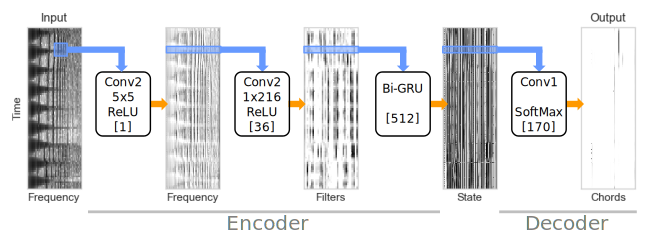
\includegraphics[width=\columnwidth]{crnn1}
    \caption{The convolutional encoder, recurrent decoder network denoted as \emph{CR1}.
            Each CQT frame is filtered by a single $5\times 5$ 2D-convolutional filter, and then encoded as a set of 36 1-D filter activations.
            The bi-directional recurrent decoder integrates across the entire observation to produce a time-series of 512-dimensional hidden state vectors. 
            Each hidden state vector is independently decoded to its most likely chord label.\label{fig:crnn1}}
\end{figure}


The convolutional feature encoding is mapped into either one or two layers of bi-directional gated recurrent units (GRUs)~\cite{cho2014learning}.
The GRU model is functionally similar to the commonly used long-short-term memory (LSTM) model~\cite{hochreiter1997long}, but has fewer parameters and often performs comparably in practice~\cite{jozefowicz2015empirical}.
For a sequence of $d$-dimensional input vectors $x(t) \in \mathbb{R}^d$, the GRU produces a sequence of $D$-dimensional hidden state vectors $h(t) \in {[-1, +1]}^D$ as follows:
\begin{eqnarray}
    r(t) &=& \sigma\left(W_r x(t) + T_r h(t-1) + b_r\right)\\
    u(t) &=& \sigma\left(W_u x(t) + T_u h(t-1) + b_u\right)\\
    \hat{h}(t) &=& \rho\left(W_h x(t) + T_h \left( r(t) \odot h(t-1) \right) + b_h \right)\label{eq:candidate}\\
    h(t) &=& u(t) \odot h(t-1) + (1-u(t)) \odot \hat{h}(t),
\end{eqnarray}
where $r(t), u(t) \in {[0,1]}^D$ are the \emph{reset} and \emph{update} vectors, each of which are controlled by RNN dynamics depending on the input $x(t)$ and previous hidden state $h(t-1)$, $\sigma$ denotes the logistic function, and $\rho$ is a non-linear activation (typically $\tanh$).
The model parameters are the input mappings $W_* \in \mathbb{R}^{D\times d}$, the state transition operators $T_* \in \mathbb{R}^{D\times D}$, and bias vectors $b_* \in \mathbb{R}^D$.

When an element of the update vector ${u(t)}_j \approx 1$, the corresponding element of the previous hidden state is copied directly to the current state ${h(t)}_j \leftarrow {h(t-1)}_j$.
Otherwise, if $r(t) \approx 1$, then $h(t)$ evolves according to standard RNN dynamics.
However, when $r(t) \approx 0$, the $h$ term in~\eqref{eq:candidate} goes to 0 and the update \emph{resets} and depends only on the input $x(t)$.
In this way, the GRU model can persist a hidden state across arbitrary long spans of time, and encode variable-length temporal dependencies.
These properties make the GRU model appealing for chord recognition, where temporal dependencies are often variable, long-range, and subject to sudden changes rather than gradual evolution.

The bi-directional variant consists of two independent GRUs, one running in each direction, whose hidden state vectors are concatenated to produce the bi-directional hidden state vector $h(t)$.
This layer integrates over the entirety of the input signal, and provides temporal smoothing and context for the encoded feature representation.

We evaluate the following decoder architectures, which trade breadth (number of hidden states) for depth (number of layers):
\begin{description}
    \item[CR1] a single Bi-GRU layer with 512 total hidden state dimensions (256 for each direction);
    \item[CR2] a stack of two Bi-GRU layers, each with 256 hidden state dimension (128 in each direction, per layer). The hidden state from the first layer is treated as input to the second.
\end{description}
While both architectures have access to the entire observation sequence, the deeper architecture may be better at capturing long-range interactions because the second layer's input has already been smoothed by the first layer.
This should allow the first layer to focus on short-term smoothing and local context, while the second layer can model chord progressions and global context.

The final hidden state vector ${h(t)}$ is decoded to the class label by a sigmoid layer, which produces a likelihood score ${\hat{y}(t)} \in {[0, 1]}^{V}$ over the chord vocabulary of $V$ symbols.
At each frame, the maximum likelihood label is selected, and the time-series of chord labels is run-length encoded to form the estimated annotation for the track.


\subsection{Chord vocabulary simplification}

\label{sec:vocab}
% For training the tag decoder, we map to a fixed vocabulary
%   1. discard missing / extra notes
%   2. discard inversions
%   3. split into (root, pitch classes)
%   4. match against quality templates:
%       - N
%       - maj, min, dim, aug
%       - min6, maj6
%       - min7, maj7, dom7, dim7, hdim7, minmaj7
%       - sus2, sus4
%       - X (unmatched)
%   5. resulting vocab = 12 * 14 + 2 = 170 classes
%

To formulate chord recognition as a classification task, we define a mapping of all valid chord descriptions to a finite vocabulary by the following procedure.\footnote{Here, a \emph{valid chord} is any string belonging to the formal language specification of Harte~\emph{et al.}~\cite{harte2005symbolic}, or the extended grammar implemented in the JAMS library~\cite{humphrey2014jams}.}
First, suppressed notes, additional notes, and inversions are discarded, \eg:
\begin{align*}
    \texttt{D}\flat\texttt{:maj(9)/3} 
    \quad\mapsto\quad \texttt{D}\flat\texttt{:maj/3}
    \quad\mapsto\quad \texttt{D}\flat\texttt{:maj}.
\end{align*}
Next, labels are decomposed into \emph{root} and \emph{pitch classes} (relative to the root) using the encoding functionality provided by \texttt{mir\_eval}~\cite{raffel2014mir_eval}, \eg:
\begin{align*}
    \texttt{D}\flat\texttt{:maj} &\mapsto \begin{cases}
        1 & \text{root}\\
        (0, 4, 7) & \text{pitch classes}
    \end{cases}.
\end{align*}
The set of active pitch classes is matched against a set of 14 templates: \texttt{min, maj, dim, aug, min6, maj6, min7, maj7, dom7, dim7, hdim7, minmaj7, sus2, sus4}.
The root and matched template are combined, and mapped to a canonical form to resolve enharmonic equivalences:
\begin{align*}
    \left(1, (0, 4, 7) \right) &\mapsto \texttt{C}\sharp\texttt{:maj}.
\end{align*}
If the pitch class set does not match one of the templates, it is mapped to the unknown chord symbol \texttt{X}; the no-chord symbol is represented distinctly as \texttt{N}.
The final vocabulary contains 170 classes: 2 special symbols (\texttt{N, X}), and $12\times14=168$ combinations of root and quality.


\subsection{Structured training}
\label{sec:encoding}

The CR models described above map each hidden state vector to a fixed vocabulary produced by the chord simplification strategy described in \Cref{sec:vocab}.
They can be optimized in the usual way by minimizing a multi-class classification loss (cross-entropy), but this approach has some clear drawbacks.

First, it does not leverage the structure of chord space.
If the model predicts \texttt{B:maj} instead of \texttt{B:7}, it is penalized just as much as if it had predicted \texttt{C:maj}.
This is at odds with evaluation (and, arguably, application utility), where predictions are evaluated along multiple dimensions, such as capturing the root, third, or fifth.
More generally, some mistakes are simply more severe than others from a transcription perspective, and this is not reflected in a 1-of-K classification formulation.

Second, the chord simplification strategy is \emph{lossy} in that it discards information such as suppressed or additional notes.
This can render certain chords ambiguous, and can introduce discrepancies between the (simplified) annotation and the corresponding acoustic content.
In the \texttt{D}$\flat$\texttt{:maj{(9)}/3} example provided in \Cref{sec:vocab}, the simplified chord \texttt{C}$\sharp$\texttt{:maj} would imply the absence of \texttt{D}$\sharp$, even though it was explicitly included in the original annotation and should be expected in the signal.
This introduces label noise to the model, and may negatively impact accuracy.

Third, out-of-gamut chords all map to a common class \texttt{X}, despite having potentially disparate tonal content.
This class provides little useful information to the model while training.
At test time, it would be beneficial if the model could predict ``nearby'' chords, but multi-class training provides little incentive to learn this behavior.


To counteract these effects, we introduce a structured representation of chords, depicted in \Cref{fig:encoding}.
This representation is inspired by the standard evaluation criteria for chord recognition, which operate over a decomposed representation of (\emph{root}, \emph{pitch classes}, \emph{bass})~\cite{raffel2014mir_eval}.
This representation can be computed for any chord in the reference annotation, and provided as a secondary supervision signal to the model, thereby helping it learn common features shared by similar chords.
At prediction time, the structured representation can be treated as output, or as an intermediate representation which contribute to the chord label prediction.


\begin{figure}[t]
    \centering
    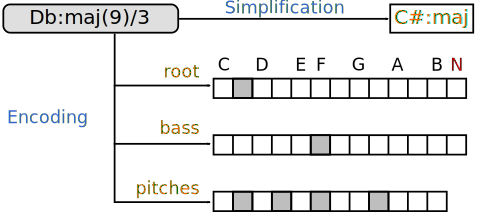
\includegraphics[width=0.9\columnwidth]{encoding}
    \caption{Target chords are represented both as simplified, canonical forms (\Cref{sec:vocab}), and as binary vectors encoding the root, bass, and pitch class content (\Cref{sec:encoding}).
    The special symbols \texttt{N,X} are mapped to an extra root/bass class denoted as \texttt{N}, and the all-zeros pitch vector.\label{fig:encoding}}
\end{figure}

The structured models (denoted as \emph{CR1/2+S}), depicted in \Cref{fig:crnn2}, predict for each frame $t$ the root pitch class (\texttt{C}--\texttt{B}, plus \texttt{N} for no-root), the bass pitch class, and the active pitch classes from the hidden state vector $h(t)$.
Root and bass estimation are modeled as a multi-class prediction with a soft-max non-linearity.
Pitch class prediction is modeled as a multi-label prediction, and uses a logistic (sigmoid) non-linearity.
This results in an idealized chroma representation similar to that of Korzeniowski and Widmer~\cite{korzeniowski2016feature}, but predicted from the hidden state of an RNN rather than a spectrogram patch.

\begin{figure}[t]
    \centering
    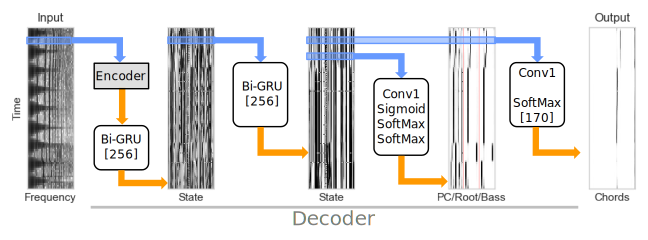
\includegraphics[width=\columnwidth]{crnn2}
    \caption{The structured convolutional encoder, recurrent decoder network, denoted as \emph{CR2+S}.
    The encoder uses the same architecture depicted in \Cref{fig:crnn2}.
    The deep decoder (\emph{CR2}) uses two bi-directional recurrent decoders to integrate information across time.
    The structured model (\emph{CR2+S}) predicts the active pitch classes, root, and bass from the second recurrent layer's hidden state.
    The hidden state, root, pitch classes, and bass predictions are then concatenated and used as inputs to the chord prediction layer.\label{fig:crnn2}}
\end{figure}

In general, it is not trivial to invert the root-chroma-bass representation to a unique chord label.
Therefore, these three layers are concatenated, along with the hidden state itself, to produce the structured representation from which the chord label is predicted.
During training, the structured models learn to minimize the sum of losses across all outputs.
In this way, the model can both leverage the structure of chord space, and learn how to decode the representation into the simplified vocabulary.

\subsection{Data augmentation}
\label{sec:muda}
To increase training set variability, we apply pitch-shifting data augmentation using MUDA~\cite{mcfee2015software}.
For each training example, 12 deformations are generated by shifting up or down by between 1--6 semitones.
Testing and validation examples are not augmented.
Because each observation exists in all twelve root classes, this provides a brute-force, approximate root invariance to the model.
Models trained with data augmentation are denoted by \emph{+A}.


\section{Evaluation}

% cite: ejh2015
%   1217, using the same 5-fold CV splits for comparison purposes
%   each training fold is split 75/25 for validation
%   training set => 12x by data augmentation
For evaluation, we used the dataset described by Humphrey and Bello~\cite{humphrey2015four}, which includes 1217 tracks from the Isophonics, Billboard, RWC Pop, and MARL collections.
To facilitate comparison with previous work, we retain the same 5-fold cross-validation splits, and randomly hold out 1/4 of each training set for validation.
We compare the proposed methods to two strong baselines: a deep convolutional network~\cite{humphrey2015four} (denoted \emph{DNN}), and the K-stream HMM~\cite{cho2014improved} (denoted \emph{KHMM}).\footnote{Comparisons were facilitated using the pre-computed outputs provided at \url{https://github.com/ejhumphrey/ace-lessons}.}

\subsection{Pre-processing}

% features
%   librosa 0.5
Feature extraction was performed with librosa 0.5.0~\cite{librosa050}.
%   log cqt power, 36bpo, (C1 - C7) (260 bins)
Each track was represented as a log-power constant-Q spectrogram with 36 bins per octave, spanning 6 octaves starting at C1, and clipped at 80dB below the peak power for the entire track.
%   sr=44100, hop = 4096 => ~96ms frame rate
Signals were analyzed at 44.1KHz with a hop length of 4096 samples, resulting in a frame rate of approximately 10.8Hz.

\subsection{Training}
% training setup
All models are trained on 8-second patches (86 frames), though the models directly generalize to arbitrarily long inputs.
For tracks with multiple reference annotations, the output is selected uniformly at random from all references for each patch.
%   8sec patches (83 frames)
%   32 patches per batch
%   512 batches per epoch
Models are trained using mini-batches of 32 patches per batch, and 512 batches per epoch.
%   ADAM optimization
We use the ADAM optimizer~\cite{kingma2014adam}, and reduce the learning rate if there is no improvement in validation score after 10 epochs.
Training is stopped early if there is no improvement in validation score after 20 epochs, and limited to a maximum of 100 epochs total.
For all models, validation score is determined solely by label prediction loss (cross-entropy).

%   validation by decoder loss
%   learning rate reduction after 10 epochs
%   early stopping after 20 epochs
%   maximum 100 epochs

%   Keras + tensorflow
All models were implemented with Keras~2.0 and Tensorflow~1.0~\cite{chollet2015keras, tensorflow2015-whitepaper}.\footnote{Source code and trained models will be made available upon publication.}

\subsection{Results}

The main results of the evaluation are listed in \Cref{fig:results}, which illustrates the median weighted recall scores achieved by each model.\footnote{The trends for the mean scores are qualitatively similar, but the scores are lower for all models. We report the median here to reduce the influence of the erroneous or otherwise spurious reference annotations reported by Humphrey and Bello~\cite{humphrey2015four}.}
\begin{figure*}[t]
    \centering
    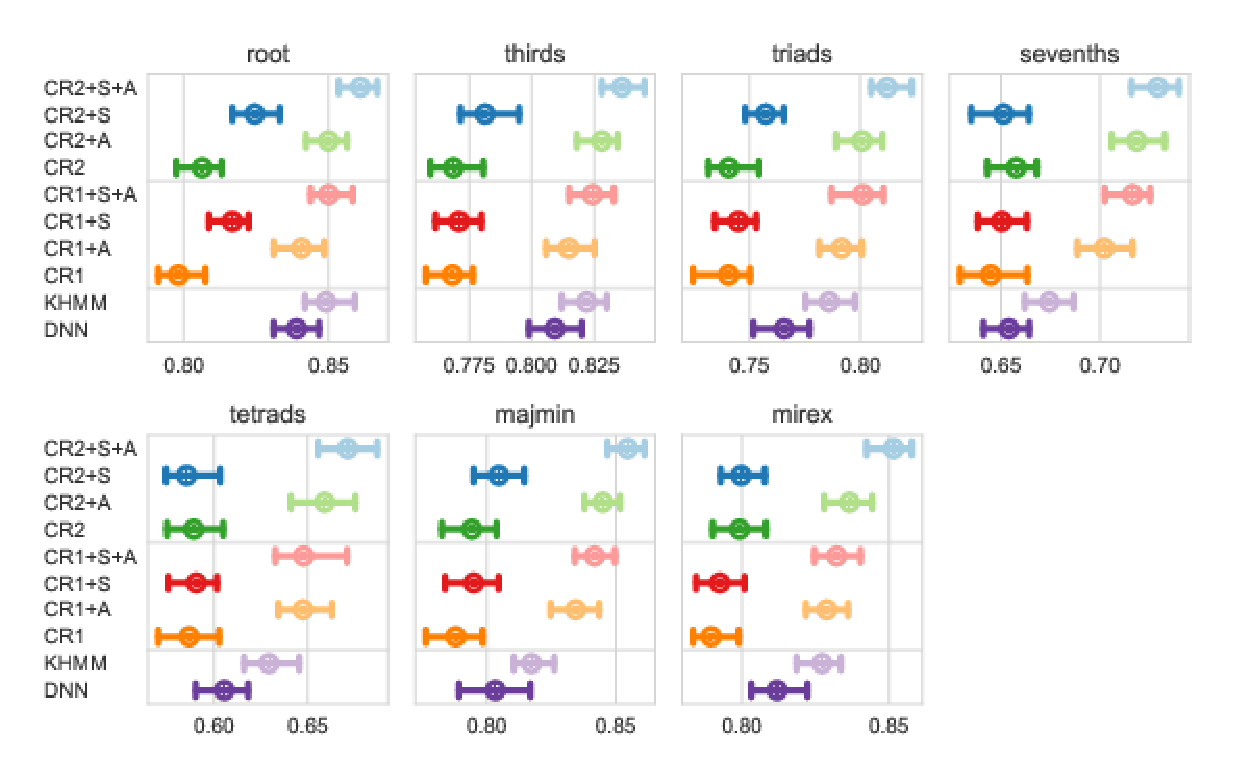
\includegraphics[width=0.9\textwidth]{crnn-scores}
    \caption{Weighted recall scores for all methods under comparison.  Each dot represents the median score across all test points, with error bars covering the 95\% confidence interval estimated by bootstrap sampling.
        \emph{KHMM} denotes the K-stream HMM of Cho~\cite{cho2014improved}; \emph{DNN} denotes the convolutional network of Humphrey and Bello~\cite{humphrey2015four}.\label{fig:results}}
\end{figure*}
Each subplot reports the recall computed by \texttt{mir\_eval} of correctly estimating the following:
\begin{itemize}
    \item \emph{root};
    \item \emph{thirds}: root and third;
    \item \emph{triads}: root, third, and fifth;
    \item \emph{sevenths}: root, third, fifth, and seventh;
    \item \emph{tetrads}: all intervals;
    \item \emph{maj-min}: 12 major, 12 minor, and \texttt{N} class; and
    \item \emph{MIREX}: at least three correct notes.
\end{itemize}

From \Cref{fig:results}, several trends can be observed.
First, data augmentation (\emph{+A} variants) provides a consistent and substantial improvement for all models.
This is to be expected, since the \emph{CR} models do not separate root from quality.
Note that DNN models root independent of quality, and KHMM was trained with chroma-rotation data augmentation, so it is unsurprising that augmentation is necessary to match performance of these methods.

Second, structured training (\emph{+S} variants) provides a modest, but consistent improvement, for both the shallow \emph{CR1} and deep \emph{CR2} decoder models.
The difference is most pronounced in the \emph{root} evaluation, which makes sense because the structured models are explicitly trained to predict the root independently of the chord label.

Third, the deep decoder models \emph{CR2} provide another small, but consistent improvement over the shallow decoders \emph{CR1}.
The aggregate scores are reported in \Cref{tab:results}; for brevity, only the models with data augmentation are included.
The combined effect of structured training, deep decoder, and data augmentation (\emph{CR2+S+A}) results in the highest scoring model across all metrics.

\begin{table*}
    \centering
    \caption{Median weighted recall scores for methods under comparison.\label{tab:results}}
    \begin{tabular}{lrrrrrrr}
        \toprule
        Method  & Root & Thirds & Triads & Sevenths & Tetrads & Maj-Min & MIREX\\
        \midrule
        CR2+S+A & 0.861 & 0.836 & 0.812 & 0.729 & 0.671 & 0.855 & 0.852\\
        CR2+A   & 0.850 & 0.828 & 0.801 & 0.719 & 0.659 & 0.845 & 0.837\\
        CR1+S+A & 0.850 & 0.824 & 0.801 & 0.716 & 0.648 & 0.842 & 0.832\\
        CR1+A   & 0.841 & 0.815 & 0.791 & 0.702 & 0.647 & 0.834 & 0.829\\
        \midrule
        KHMM~\cite{cho2014improved}    & 0.849 & 0.822 & 0.785 & 0.674 & 0.629 & 0.817 & 0.827\\
        DNN~\cite{humphrey2015four}     & 0.838 & 0.809 & 0.766 & 0.654 & 0.605 & 0.803 & 0.812\\
        \bottomrule
    \end{tabular}
\end{table*}
\subsection{Error analysis}

To get some more insight about the mistakes made by the model at test time, we illustrate the frame-wise, within-root quality confusion matrix for the \emph{CR2+S+A} model in \Cref{fig:confusion}.
For each frame of a test track, its true (simplified) label is compared to the label predicted by the model if they match at the root.
Results are then aggregated across all test tracks, and normalized by (reference quality) frequency to produce the confusion matrix.
Under this evaluation, the \emph{CR2+S+A} achieves 63.6\% accuracy of correctly identifying the simplified chord label (root and quality) at the frame level.

\begin{figure}
    \centering
    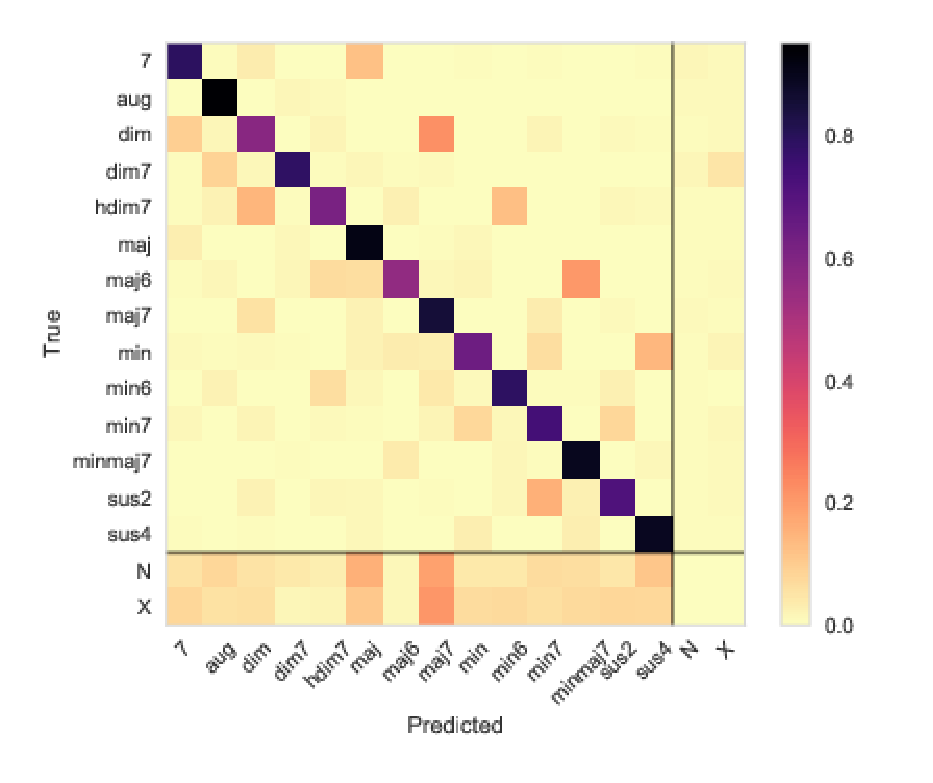
\includegraphics[width=\columnwidth]{qualconf}
    \caption{Within-root, frame-wise quality confusions for the best performing model \emph{CR2+S+A}.
    The value at row $i$ column $j$ corresponds to fraction of frames labeled as class $i$ but predicted as class $j$.
    Results are aggregated across frames over all test tracks.\label{fig:confusion}}
\end{figure}

In \Cref{fig:confusion}, the first obvious trend is a bias toward \texttt{min} and \texttt{maj}, in accordance with the natural bias in the training set.
Note, however, that the confusions are generally understandable as simplifications of true labels, \eg, \texttt{min7}$\rightarrow$\texttt{min} and (\texttt{maj7},\texttt{7})$\rightarrow$\texttt{maj}.
The model still appears to struggle with 6th and suspended chords, which account for 1.5\% and 2.5\% of the data (by duration), respectively.
The bottom row corresponds to out-of-gamut \texttt{X}-chords, which map overwhelmingly to \texttt{maj} and \texttt{min}.
This can be explained by examining which labels map to \texttt{X} during simplification.
There are 4557 instances of such chords in the corpus (2.2\% of the data), and of these, 2091 are 1-chords (only the root) and 2365 are power chords (root+fifth), neither of which map unambiguously onto the simplified vocabulary.
The model appears to be resolving these points toward the more commonly used \texttt{min} and \texttt{maj} qualities.

\begin{figure}
    \centering
    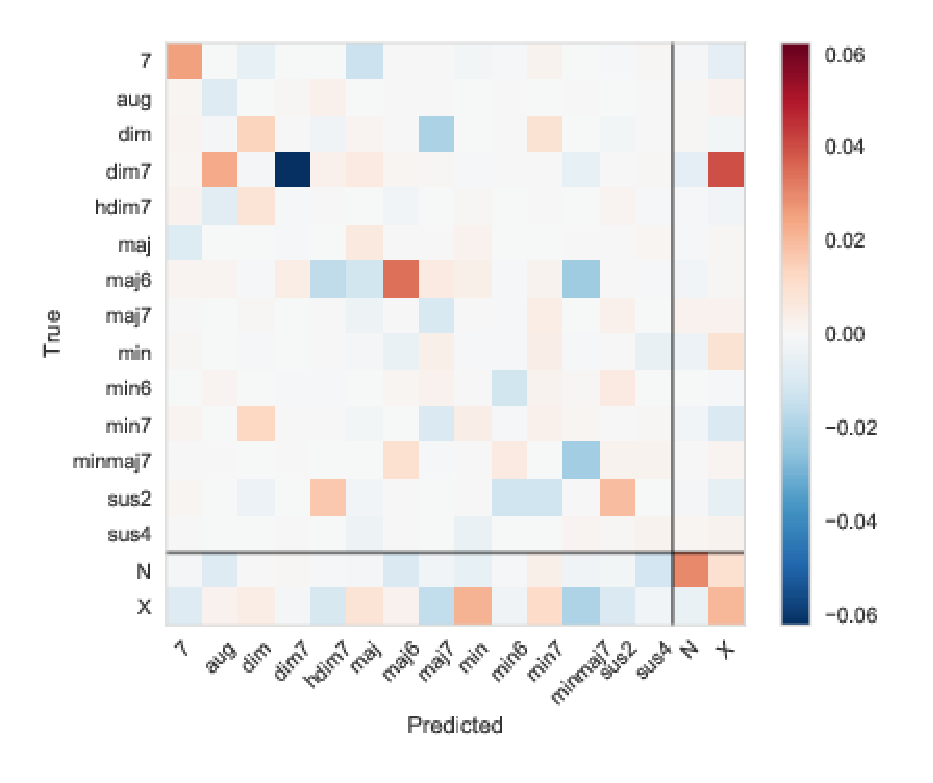
\includegraphics[width=\columnwidth]{confdelta}
    \caption{The difference between confusion matrices for \emph{CR2+S+A} and the unstructured \emph{CR2+A} (best viewed in color).
    Positive values along the diagonal indicate increased accuracy for \emph{CR2+S+A}.\label{fig:confdelta}}
\end{figure}

For comparison purposes, the difference in the confusion matrices between the structured model \emph{CR2+S+A} and the unstructured model \emph{CR2+A} is depicted in \Cref{fig:confdelta}.
Here, positive values (red) along the diagonal indicate increased accuracy for the structured model, while negative values along the diagonal (blue) indicate decreased accuracy.
The net effect is positive, increasing accuracy by +0.8\% over \emph{CR2+A}, which achieves accuracy of 62.8\%.

Despite a slight degradation in accuracy for \texttt{maj7}, there is a substantial increase in accuracy for \texttt{aug}, \texttt{dim7}, \texttt{hdim7}, and modest improvement for \texttt{sus4}.
Moreover, there is a consistent reduction of confusions to \emph{maj}, illustrated by the negative values in the second column, which indicates that the structured model is more robust to quality bias in the training set.
Compared to the unstructured model, the structured model reduces confusions from \texttt{aug} to (\texttt{maj}, \texttt{7}), and \texttt{dim7} to (\texttt{min}, \texttt{7}, \texttt{N}).
While \emph{CR2+S+A} still performs poorly on the rarest class \texttt{minmaj7} (0.03\% of the data), compared to \emph{CR2+A}, it resolves toward \texttt{min} more often and \texttt{min7} less often.
This indicates that the structured model is better at abstainining from predicting a seventh if it appears unlikely, rather than predict it in the wrong position.


\section{Conclusion}
This work developed deep architectures and a structured training framework for chord recognition in large vocabularies.
Although the proposed model improve over the baseline methods, there are clear directions forward in extending the ideas presented here.
First, although the proposed model predicts the bass note, this feature is only used for establishing context in decoding, and the model does not predict inversions.
Supporting inversion prediction would be a simple extension of the method described here, and would not require creating special vocabulary entries for each potential inversion.
Second, the structured representation facilitates modeling infrequently observed, complex chords, and could readily be extended to support extended chords by using a multi-octave pitch class representation.
However, doing so effectively---and evaluating the resulting predictions---would require larger annotated corpora for these classes than are presently available.

%   future work
%       expanded vocab
%           1/5 chords
%           extensions above the octave --> two-octave ideal chroma
%           this will require larger annotated corpora for these categories to be worthwhile though
%       bass tracking
%       


%\section*{Acknowledgments}

% For bibtex users:
\bibliography{refs}

\end{document}
